\documentclass[acmtog]{acmart}

\usepackage{booktabs} % For formal tables

% TOG prefers author-name bib system with square brackets
\citestyle{acmauthoryear}
%\setcitestyle{nosort,square} % nosort to allow for manual chronological ordering



\usepackage[ruled]{algorithm2e} % For algorithms
\renewcommand{\algorithmcfname}{ALGORITHM}
\SetAlFnt{\small}
\SetAlCapFnt{\small}
\SetAlCapNameFnt{\small}
\SetAlCapHSkip{0pt}

% Metadata Information
\acmJournal{TOG}
\acmYear{2019}\acmVolume{38}\acmNumber{4}\acmArticle{1}\acmMonth{7} \acmDOI{10.1145/3355089.3356531}

% Copyright
\setcopyright{acmcopyright}

% Paper history
%\received{February 2007}
%\received{March 2009}
%\received[final version]{June 2009}
%\received[accepted]{July 2009}

% !TEX root =  ShapeSpaceDog.tex

\usepackage{amsmath}
\usepackage{amssymb}
\usepackage{amsfonts}
\usepackage{enumitem}
\usepackage[mathscr]{eucal}
%\usepackage[ruled,vlined]{algorithm2e}
\usepackage{algorithmic}
\usepackage{microtype}
\usepackage{units}


% compact bullet lists and enumeration environments
\newenvironment{tight_enumerate}{
\begin{enumerate}[topsep=4pt,itemindent=\parindent]
  \setlength{\itemsep}{1pt}
  \setlength{\parskip}{0pt}
  \setlength{\parsep}{0pt}
}{\end{enumerate}}

%\newenvironment{tight_itemize}{
%\begin{itemize}[topsep=4pt]
%  \setlength{\itemsep}{1pt}
%  \setlength{\parskip}{0pt}
%  \setlength{\parsep}{0pt}
%}{\end{itemize}}


\usepackage{dsfont}
\usepackage{graphicx,wrapfig}

\usepackage{mdframed}
\mdfsetup{skipabove=\topskip,skipbelow=\topskip}
\newmdenv[	linewidth=0.75pt,
			leftline=false,
			rightline=false,
   			innerleftmargin=0pt,
			innerrightmargin=0pt]{topbot}

%\usepackage[mathcal]{euscript}

%\usepackage{amsthm}
%\newtheorem{theorem}{Theorem}[section]
%\newtheorem{lemma}[theorem]{Lemma}
%\newtheorem{proposition}[theorem]{Proposition}
%\newtheorem{corollary}{Corollary}
\newtheorem{mydefinition}{Definition}

\newcommand{\MiR}[1]{{\bf\textcolor{cyan}{MR: #1}}} % Michael
\newcommand{\OSH}[1]{{\bf\textcolor{red}{OSH: #1}}} % Olga
\newcommand{\TimH}[1]{{\bf\textcolor{blue}{TH: #1}}} % Tim 
\newcommand{\Rev}[1]{{#1}} % Revision

\newcommand{\todo}[1]{{\bf\textcolor{red}{TODO: #1}}}

%\newcommand{\newt}[1]{{\textcolor{blue}{#1}}}
\newcommand{\newt}[1]{{#1}}


%Abbreviations
\newcommand{\figref}[1]{Fig.\ \ref{#1}}
\newcommand{\secref}[1]{Sec.\ \ref{#1}}
\newcommand{\appref}[1]{Appendix \ref{#1}}
\newcommand{\equref}[1]{Eq.\ \eqref{#1}}
\newcommand{\defref}[1]{Def.\ \ref{#1}}
\newcommand{\lemmaref}[1]{Lemma \ref{#1}}
\newcommand{\theoremref}[1]{Theorem \ref{#1}}
\newcommand{\corollaryref}[1]{Cor.\ \ref{#1}}


% operators
\DeclareMathOperator*{\argmin}{arg\,min}
\DeclareMathOperator*{\argmax}{arg\,max}
\DeclareMathOperator*{\Proj}{Proj}


% Olga SH notation
\newcommand{\set}[1]{\mathcal{#1}}
% Transpose symbol
\newcommand{\transposeSign}{\textsf{T}}
\newcommand{\tr}{\transposeSign}


\newcommand{\R}{\mathds{R}}
\newcommand{\Z}{\mathds{Z}}
\DeclareMathOperator{\atantwo}{atan2}

\newcommand{\x}{x}
\newcommand{\p}{p}

\newcommand{\Fbo}{F_{\bar{1}}}
\newcommand{\Fbt}{F_{\bar{2}}}

\newcommand{\FAll}{\mathbf{F}}
\newcommand{\II}{I\!I}
\newcommand{\Atotal}{\mathcal{A}}


%\renewcommand{\ra}{\rightarrow}
\newcommand{\norm}[1]{\left\Vert#1\right\Vert}
\newcommand{\Norm}[1]{\lvert \! \lvert \! \lvert #1 \rvert \! \rvert \! \rvert}
\newcommand{\abs}[1]{\left\vert#1\right\vert}
\newcommand{\babs}[1]{\Big \vert#1 \Big \vert}
\newcommand{\bra}[1]{\left\{#1\right\}}
\newcommand{\parr}[1]{\left (#1\right )}
\newcommand{\brac}[1]{\left [#1\right ]}
\newcommand{\ip}[1]{\left \langle #1 \right \rangle }
\newcommand{\eps}{\varepsilon}


\newcommand{\alter}[1]{\textcolor{magenta}{[Alt: #1]}}
\newcommand{\opt}[1]{\textcolor{magenta}{[Opt: #1]}}
\newcommand{\rem}[1]{\textcolor{magenta}{[Rem: #1]}}

\newcommand{\LP}{\mathbb{L}}
\newcommand{\J}{\mathbf{J}}
\newcommand{\K}{\mathbf{K}}
\newcommand{\D}{\mathscr{D}}
\newcommand{\GR}{{\mathcal{G}}}
\newcommand{\I}{{\mathcal{I}}}
\newcommand{\CO}{\mathcal{C}}
\newcommand{\GI}{{\GR}_{\I}}
\newcommand{\GC}{{\GR}_{\CO}}
\newcommand{\M}{\mathcal{M}}
\newcommand{\Mevo}{{\M}_{evo}}
\newcommand{\Mgen}{{\M}_{G}}
%\newcommand{\u}{\mathscr{u}}
%\newcommand{\v}{\mathscr{v}}
\newcommand{\TD}{\ensuremath{T_{F}\D}}
\newcommand{\ND}{\ensuremath{N_{V(t)}\D}}
% Document starts
\begin{document}
% Title portion
\title{Modeling Curved Folding with Freeform Deformations}

% Authors.
\author{Michael Rabinovich}
\affiliation{%
  \institution{ETH Zurich}
  \department{Department of Computer Science}
  \streetaddress{Universit\"atstrasse 6}
  \city{Zurich}
  \postcode{8092}
  \country{Switzerland}}
\author{Tim Hoffmann}
\affiliation{%
  \institution{TU Munich}
  \department{Department of Mathematics}}
\author{Olga Sorkine-Hornung}
\affiliation{%
  \institution{ETH Zurich}
  \department{Department of Computer Science}
  \streetaddress{Universit\"atstrasse 6}
  \city{Zurich}
  \postcode{8092}
  \country{Switzerland}}
% This command defines the author string for running heads.
\renewcommand{\shortauthors}{Rabinovich, Hoffmann, Sorkine-Hornung}

% A "teaser" figure, centered below the title and authors and above the body of the work.
\begin{teaserfigure}
  \centering
  \includegraphics[width=\linewidth]{figures/teaser_1}
  \caption{\label{fig:teaser} Curved folded surfaces modeled with our method, along with their crease patterns. Our deformation algorithm is able to simultaneously bend and fold complicated crease patterns using only positional constraints, while automatically finding a valid mountain/valley assignment along the creases. Our framework is suitable for freeform editing and exploration of new curved folded surfaces.
}
\end{teaserfigure}
\begin{abstract}
% !TEX root =  CurvedFoldedDogs.tex
We present a computational framework for interactive design and exploration of curved folded surfaces, which is typically done in a manual physical process. Our objective is to lay the foundations for the digitalization of curved folded surface design.
We base our approach on modeling the shapes using discrete orthogonal geodesic nets (DOGs) in a piecewise manner. DOGs are used to represent the smooth parts of the modeled shape, and we connect different DOGs along curves that represent the sharp creases and folds. 
%, based on piecewise discrete orthogonal geodesic nets (DOGs). 
Our main 
%apparatus 
contribution is a discrete binary characterization for folds between DOGs, accompanied by an algorithm to simultaneously fold creases and smoothly bend planar sheets. We complement our algorithm with essential building blocks for curved folding deformations: objectives to control dihedral angles and mountain-valley assignments. We apply our machinery in a curved folding editing system, thus building the first tool capable of modeling bending and folding of complicated crease patterns.

% and explore areas previously uncharted by computer simulations such as wallpaper curved folding, as well as dynamically adding, removing, and moving creases along a flattened pattern.
\end{abstract}


%
% The code below should be generated by the tool at
% http://dl.acm.org/ccs.cfm
% Please copy and paste the code instead of the example below.
%
\begin{CCSXML}
<ccs2012>
<concept>
<concept_id>10010147.10010371.10010396.10010397</concept_id>
<concept_desc>Computing methodologies~Mesh models</concept_desc>
<concept_significance>500</concept_significance>
</concept>
<concept>
<concept_id>10010147.10010371.10010396.10010398</concept_id>
<concept_desc>Computing methodologies~Mesh geometry models</concept_desc>
<concept_significance>500</concept_significance>
</concept>
</ccs2012>
\end{CCSXML}

\ccsdesc[500]{Computing methodologies~Mesh models}
\ccsdesc[500]{Computing methodologies~Mesh geometry models}

%
% End generated code
%


\keywords{curved folding, developable surfaces, discrete differential geometry, geodesic nets, shape modeling}



\maketitle
\section{Introduction}
There are myriads of ways to deform a planar sheet without stretching or tearing it. One can bend it, fold it, or combine the two. Folding and bending isometries are different by nature, and historically speaking there is some dichotomy in the study of the two; Smooth isometries are typically studied in differential geometry \cite{do_carmo}, whereas straight folds are often explored in the field of computational origami \cite{origami_book}. Curved folded surfaces \cite{huffman} results from a combination of the two, as folding an inextensible sheet along a curve necessitates global bending around the crease.

Building curved folded sculptures is a manual and time consuming process, often done using an empirical trial and error approach  as little theory is known \cite{curved_review,huffmann_reconstructing}. Contrary to classical origami, bending and folding instructions are hard to write down and the fact that multiple creases need to fold simultaneously further complicates the process \cite{StringActuated:2017}. In practice, artists often pre-crease the paper using a ball burnisher or a CNC plotter before carefully folding and bending it.

Albeit manual, slow, and exhaustive, playing with paper is currently the only option available for an explorer of curved folds. Existing works on modeling these surfaces are either limited to previously discovered sculptures \cite{curved_folding_kilian,StringActuated:2017} or model a small partial set of folded surfaces generated by reflections or rotational sweeps \cite{Mitani_ref,mitani2009design}. Modeling the folding process of novel forms remains a challenge \cite{curved_review}. In this paper we set to develop the basic tools for unconstrained modeling of curved folds, in order to aid the exploration, analysis and study of new curved folded structures.

Our work builds upon Discrete Orthogonal Geodesic Nets (DOGs) \cite{rabi18,rabi2018shape} as a discrete model for smooth developable surfaces parameterized by orthogonal geodesics. These are regular quadrilateral meshes with equal angles around each vertex, and unlike other computational models for developables do not suffer from locking of various deformation modes \cite{locking1,locking2,grin_shells}, are not fixed to predetermined rulings directions \cite{pottmann_new,curved_folding_kilian} or require remeshing while deforming the surface \cite{StringActuated:2017,SchreckEG2017,Narain}. We represent curved folded models as piecewise smooth developable surfaces with tangent discontinuities and equal geodesic curvature along their intersections, as done in \cite{rabi2018shape}. 

% Bifurcation mode... Explains that it doesn't have to fold, and it is more complicated when there are more folds, and hence one needs to give a simple definition and algorithm for folding. Then continue that there are other parameters one would like to control such as angles and rulings, and bla bla.
The challenge is then to find deformations that leads to a folded configuration (ADD:FIGURE).

% There are 2 components for such modeling. The first is a good model, the second is a way to navigate and fold that model, similarly as to how one needs to place is fingers in order to fold a piece of paper. We use the model


% The beautiful art of curved folded sculptures is almost a hundred years old, dating back to the 1920's works of Josef Albers in the Bauhaus art school \cite{josef_albers_thesis}, and continuing with the investigations of David Huffman and Ron Resch in the 1970's \cite{huffman,resch1974portfolio}. 

% Many of these early works, are mathematically not yet fully understood. We know what happens in one fold, but multiple ones still forms a challenge and we only have specific investigation for some cases. Creating them is , using paper and They date to 1920's but we only know what happen along one fold, or analyze specific set of examples, and don't know how typical models even fold. Computer simulations of that can help, but are somehow legging behind what is mostly experimented by hand, in a process that is in fact time consuming, often involving using a pen bla and da da da.

\section{Related work}
\subsection{Modeling developable surfaces}
A smooth surface is called a \textit{developable surface} if it is locally isometric to the plane, or equivalently has zero Gaussian curvature. Though well understood mathematically \cite{do_carmo,spivak,computational_line}, there is a plethora of work on modeling developable surfaces, which has been proven to be a challenge. The primary difficulty lies in using a discrete model that is able to capture the full set of deformations keeping a surface developable. These include extrinsic deformations as well as intrinsic deformations. The latter stretch a surface while keeping it developable, and is used for geometry exploration tasks where the size and shape of the flattened developable surface is unknown \cite{conical,pottmann_new,rabi2018shape}. A failure of a discrete model to discretize the full range of smooth deformations is often termed \textit{locking} \cite{solomon,locking1} and is the bane of most discrete developable models. Ruling based models \cite{conical,curved_folding_kilian,pottmann_new,stein_dev,solomon} are limiteds to a partial set of extrinsic deformations while isometry based methods \cite{grin_shells,shells, goldenthal2007efficient,froh_botsch} do not model intrinsic deformations by design, but are also prone to locking of various bending deformations \cite{locking1,locking2}, and are often coupled with dynamic remeshing \cite{narain2012adaptive,StringActuated:2017,Narain,SchreckEG2017}. \MiR{should I explicitly say that remeshing is complicated and is also not backed up by any theory?} Our work is based on modeling a developable surface as a discrete orthogonal geodesic net (DOG) \cite{rabi18}, a model that have been shown both theoretically and empirically to avoid extrinsic or intrinsic deformations locking. We further rely on \cite{rabi2018shape} to deform and explore the shape space of DOGs, but replace the authors' Laplacian flow deformation with an SQP algorithm as further detailed in \secref{sec:implementation}.
\subsection{Curved folding}
The beautiful art of curved folded sculptures is almost a hundred years old, dating back to the 1920's works of Josef Albers in the Bauhaus art school \cite{josef_albers_thesis}, and continuing with the investigations of David Huffman and Ron Resch in the 1970's \cite{huffman,resch1974portfolio}. This art, though intimately linked to the mathematics of developable surfaces, is mostly driven by physical experiments with paper \cite{curved_review}. As opposed to smooth developable surfaces \cite{do_carmo} or straight fold origami \cite{origami_book}, the mathematics of curved folding is legging behind the manual craft, and mostly concerns the local behavior of a single folded curved crease \cite{duncan_folded,mathematical_omnibus,curved_review}. Notable crease patterns such as the Huffmann Tower \cite{huffman2,huffmann_reconstructing}, are not yet understood \cite{demaine2018conic} and the known mathematics on folding and bending multiple curved creases is limited to a very few particular cases, coupled with a specific folding movement and guided by fixed rulings \cite{demaine_lens, demaine2018conic}. In essence, we do not know much about which crease patterns fold, and we do not know in which ways they can fold; Unlike straigh origami, there are often infinite ways of folding bending a curved crease pattern by varying the dihedral angles as well as the developable rulings along different creases. \\
Curved folding was first introduced to the geometry processing community by work of \cite{curved_folding_kilian}, who reconstructed scanned curved folded surfaces. In \cite{StringActuated:2017} the authors simplify the process of fabrication of curved folded models using a string actuation network. Both of these works assume an access to known target surfaces. Other works on modeling developable surfaces focus on a given subset of folds, such as planar creases generated by reflection \cite{mitani2012column,Mitani_ref}, surfaces generated by rotational sweeps \cite{mitani2009design}. The works \cite{pottmann_new} model curved folded surfaces with a rigid ruling pattern. We note that the majority of curved folding deformations change the rulings throughout the folding process. 
% Write that the only system of freeform exploration of curved folding that the authors know of is based on DOGs, that this hits a limit with multiple creases and that we extend upon that work (refer to fig 2 again).
\section{Setup} \label{sec:setup}
\subsection{Definitions}
Throughout the paper, we use the following definition for a curved folded surface:
\begin{definition} \label{def:curved_folded_surface}
A surface $S$ is called a curved folded surface if it is locally isometric to the plane and can be written as $S = \bigcup P_i $ where each $P_i$ is a $C^2$ developable surfaces termed a \textit{patch}, and their intersections $P_i \cap P_j$ are $C^2$ curves.
\end{definition}
% consists piecewise $C^2$ developable surface whose discontinuities are focused along $C^2$ curves. More formally, 
This definition is suitable for various topologies, such as a cylinder, although throughout the paper we will work with surfaces that can be globally isometrically flattened to the plane. Borrowing terms from \cite{origami_book,non_pleated}, we often refer to the surface \textit{crease pattern} consisting of the planar isometric surface domain $S_P$ together with the flattened intersection curves between the interior of the patches $P_i$ (see \figref{fig:crease_pattern}). The flattened domain boundaries together with the flattened intersection curves form a (pseudoline) planar arrangement \cite{arrangements}, inducing a planar graph decomposing $S_p$ into different disconnected components termed faces, which are domains isometric to the patches $P_i$. The vertices of this graph are the intersection of the curves with each other or the boundary curves, which we call \textit{crease vertices}. The \textit{edges} of this graph are curves isometric to the intersections of the various patches (see \figref{fig:crease_pattern}), and we refer to the inner points of these curves as \textit{crease points}, i.e. points on these curves that are not \textit{crease vertices}. We say that $S$ is \emph{folded} along a crease point if at this point the patches $P_i,P_j$ sharing it has a tangential discontinuity (see \figref{fig:folded_and_not_folded}).

\begin{figure} [h]
	\centering
	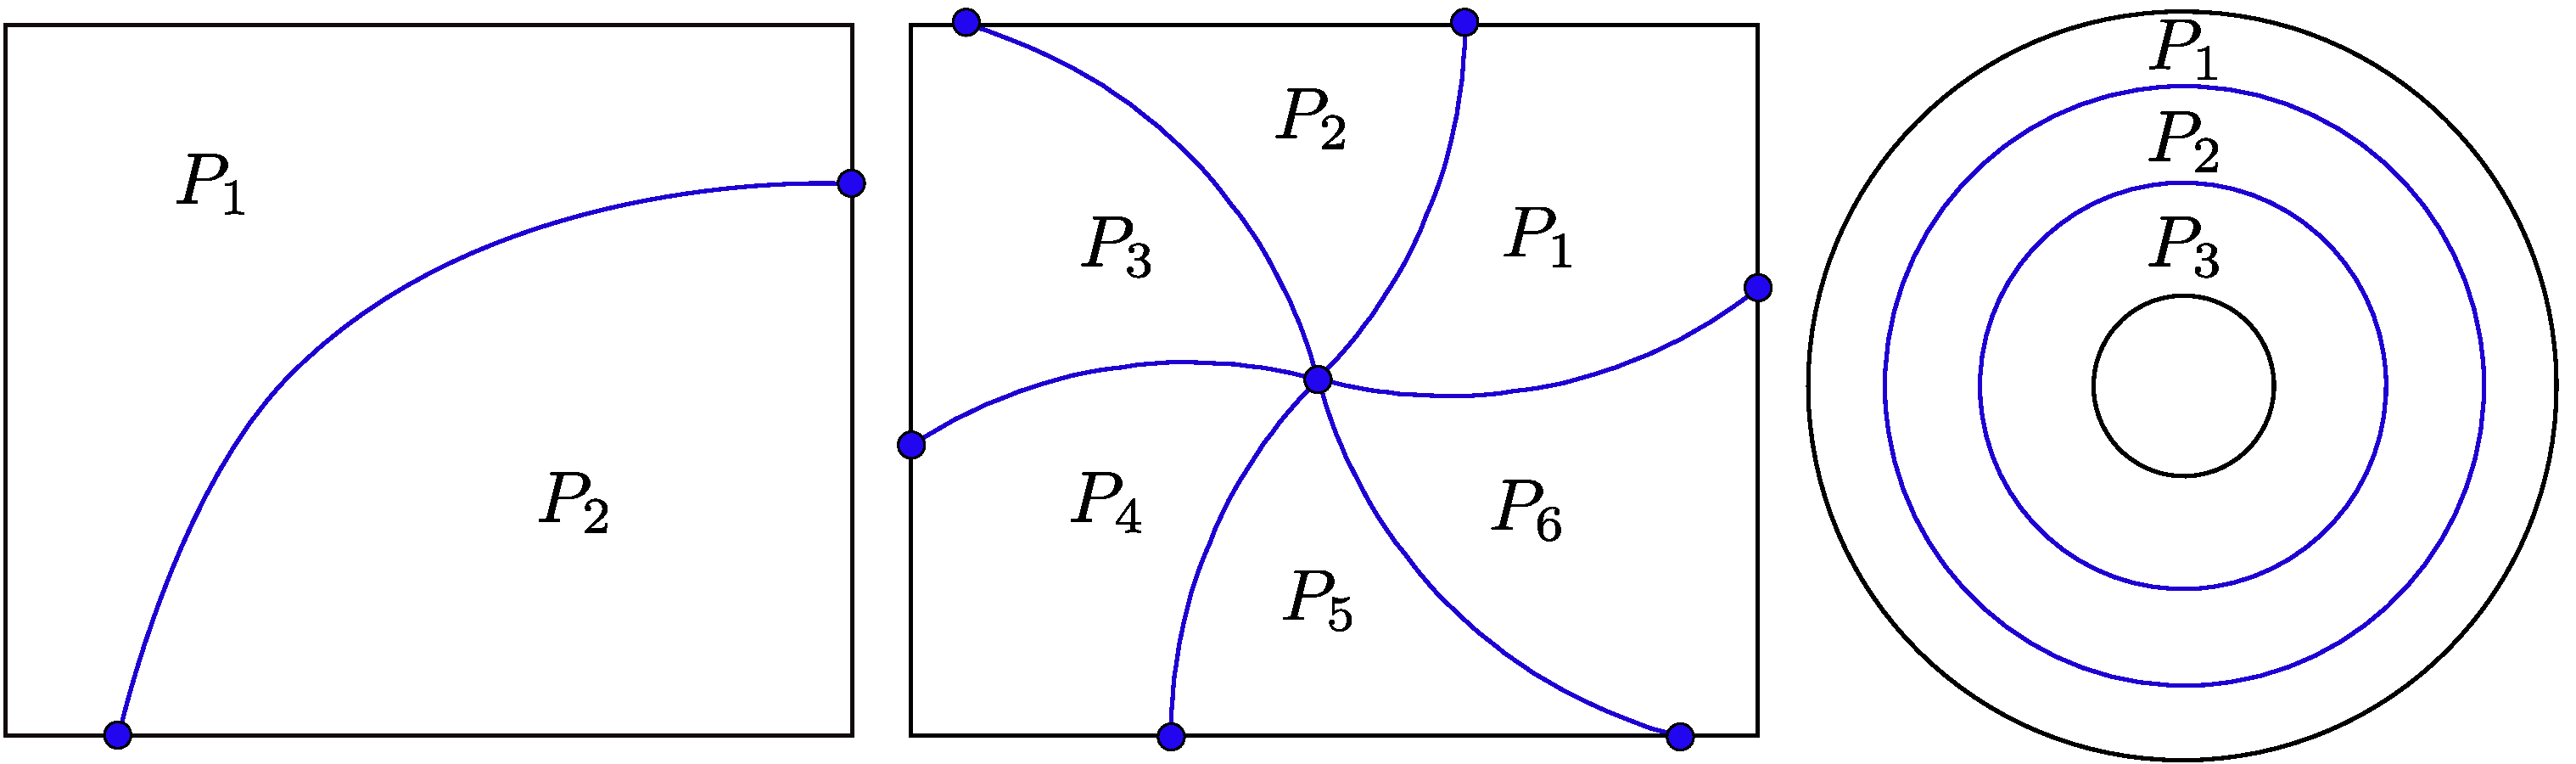
\includegraphics[width=\linewidth]{figures/crease_patterns}
	\caption{Curved crease patterns, decomposing a pattern into multiple components $P_i$ and intersecting at crease vertices. Boundary curves in black, crease curves in blue.}
	\label{fig:crease_pattern}
\end{figure}
We are interested in deformations on curved folded surfaces that keeps them curved folded. Viewed separately on each patch $P_i$, these deformation are $C^2$, though they often introduce tangent discontinuities along the patches intersections. At \cite{demaine_lens} the authors refer to creases that remain $C^2$ as \textit{smoothly folded} creases (though they define it as $C^1$ they prove that this implies that they are $C^2$). In particular we are interested in such continuous deformations, or deformation flows \cite{rabi2018shape}, which we refer to as curved folding flows. We denote these flows by a continuous map $S(t), 0 \leq t \leq 1$, where each $S(t)$ is a curved folded surface and the flow is $C^2$ when limited to each patch. We often look at the case where the starting point $S(0)$ planar. In this paper we focus on modeling isometric curved flows, which we also refer to as \emph{folding}. These flows can can be used to model physical paper or metal folding, though most of our observations and tools can also be used to model curved folding flows that are not isometries. Non-isometric developable deformations can be useful for design tasks where the a-priori flattened shape is unknown \cite{rabi18,rabi2018shape} .

\subsection{Model} \label{sec:model}
We follow the work of \cite{rabi2018shape} by modeling each patch $P_i$ as a discrete orthogonal geodesic net (see \figref{fig:curve_on_dog}). We represent a crease as piecewise linear curves, whose points $c(i)$ are represented by the curves' intersection point with the grid edges. Each point $c(i)$ is a linear combination of two vertices on a DOG: $c(i) = t v_i + (1-t)v_j,$ where $0 \leq t \leq 1$ and $v_i,v_j$ are too neighbour vertices on the grid.  Each point on a crease lies on each of the $m \geq 2$ different patches, essentially duplicated. If $c(i)^1,c(i)^2,....,c(i)^m$ are the representation of $c(i)$ on the different patches, we enforce constrain these duplicated points have equal coordinates (see \figref{fig:curve_on_dog}).
We trivially extend the represntation at \cite{rabi2018shape} to support intersecting curves by adding grid lines at crease vertices (see \figref{fig:piecewise_dog_from_crease} and \figref{fig:curve_on_dog}).

\begin{figure} [h]
	\centering
	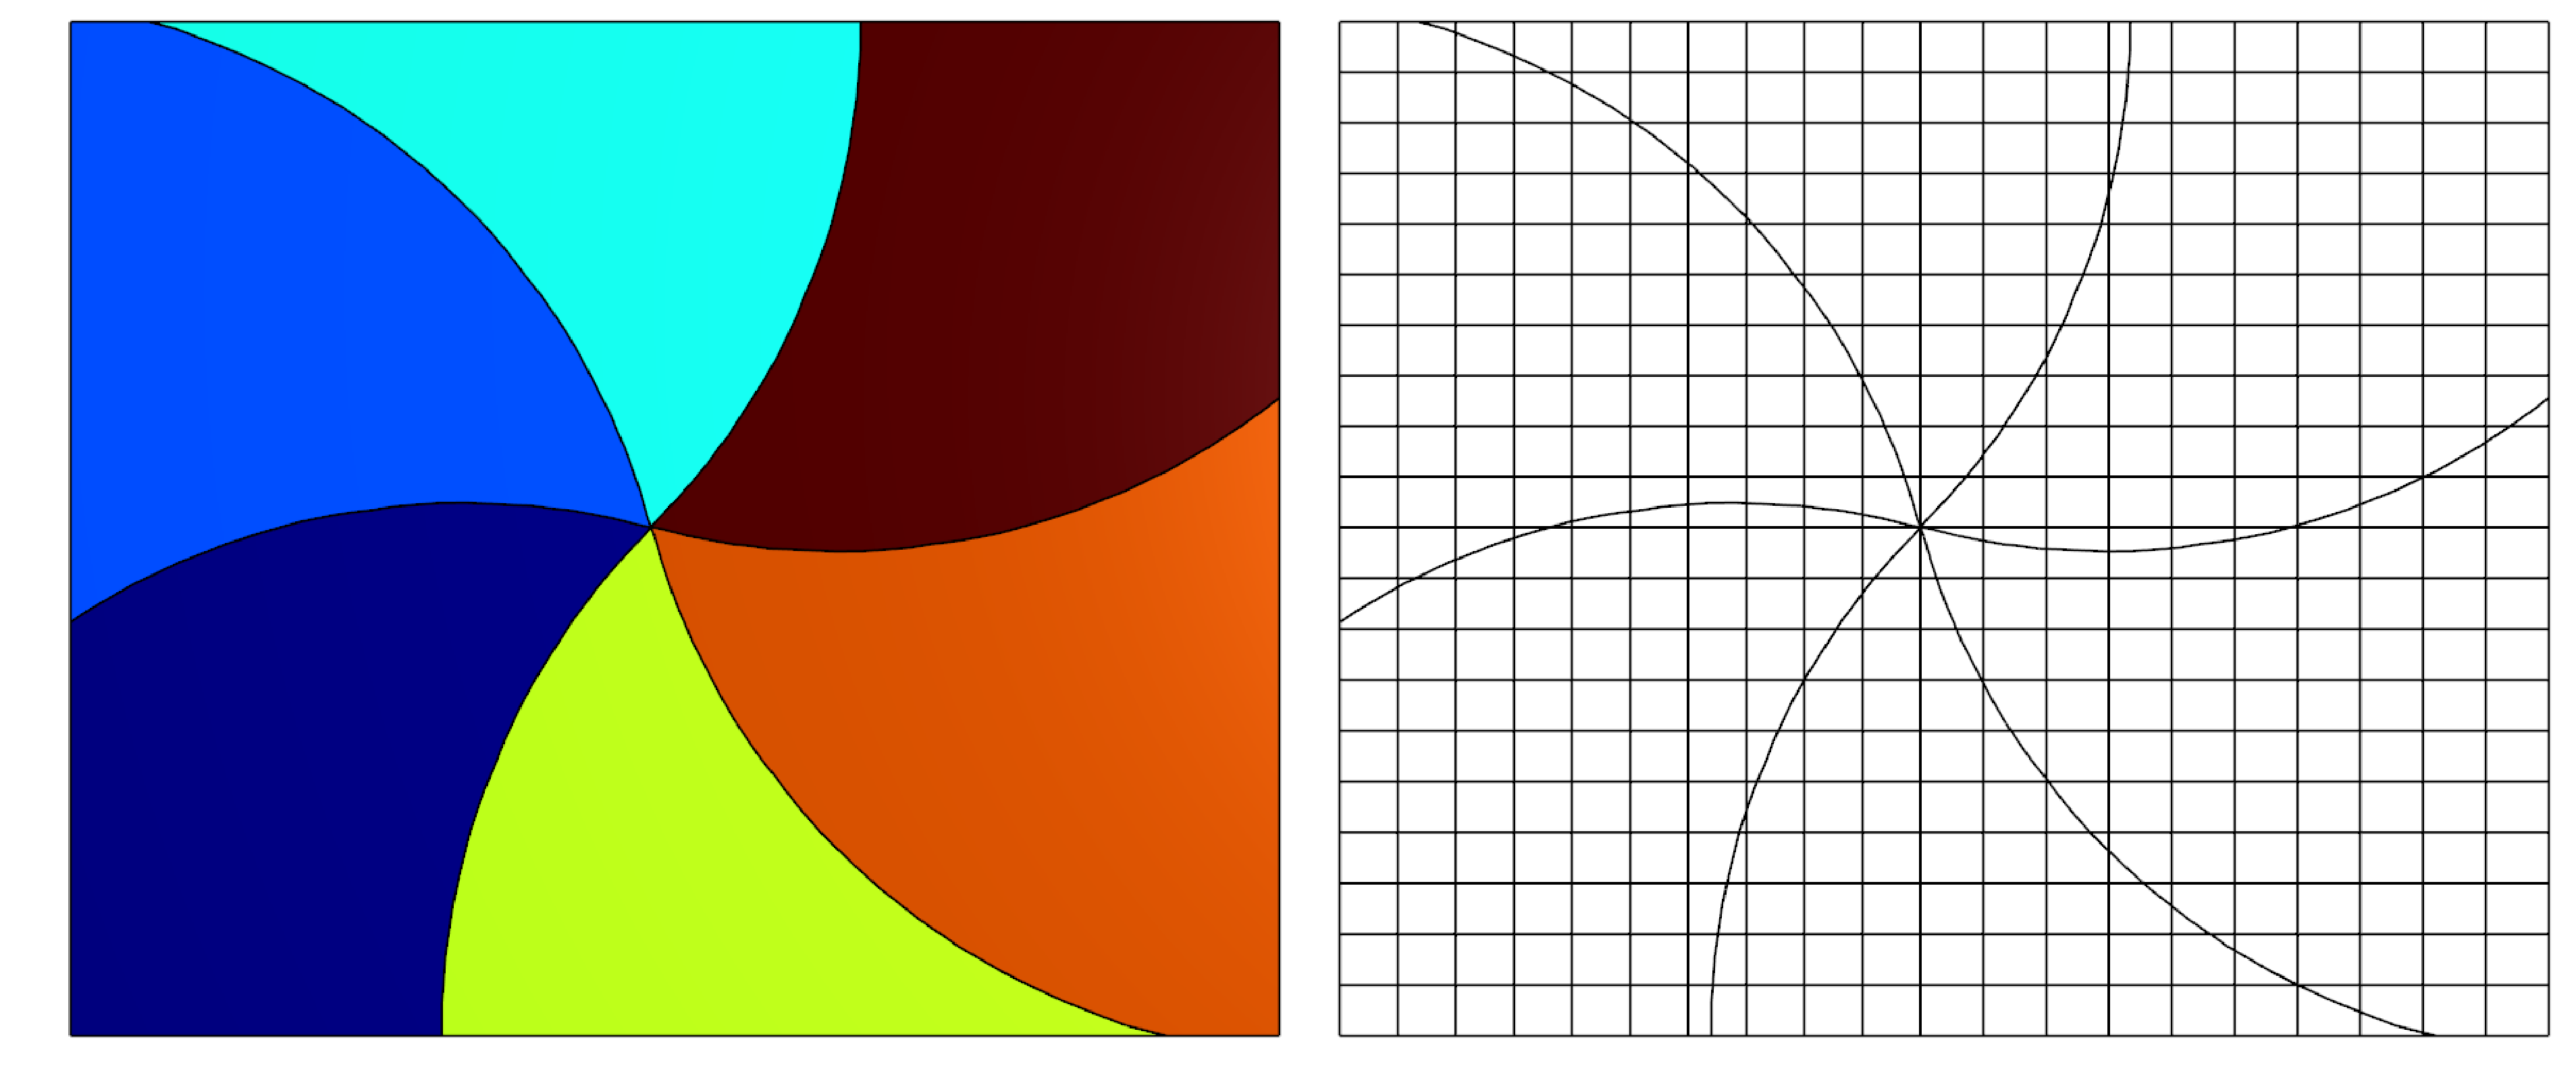
\includegraphics[width=0.8\linewidth]{figures/piecewise_dog_from_crease}
	\caption{Given a crease pattern, we create a DOG for each segment (colored differently), and use the boundary constraints as done in \cite{rabi2018shape}.}
	\label{fig:piecewise_dog_from_crease}
\end{figure}

\begin{figure} [h]
	\centering
	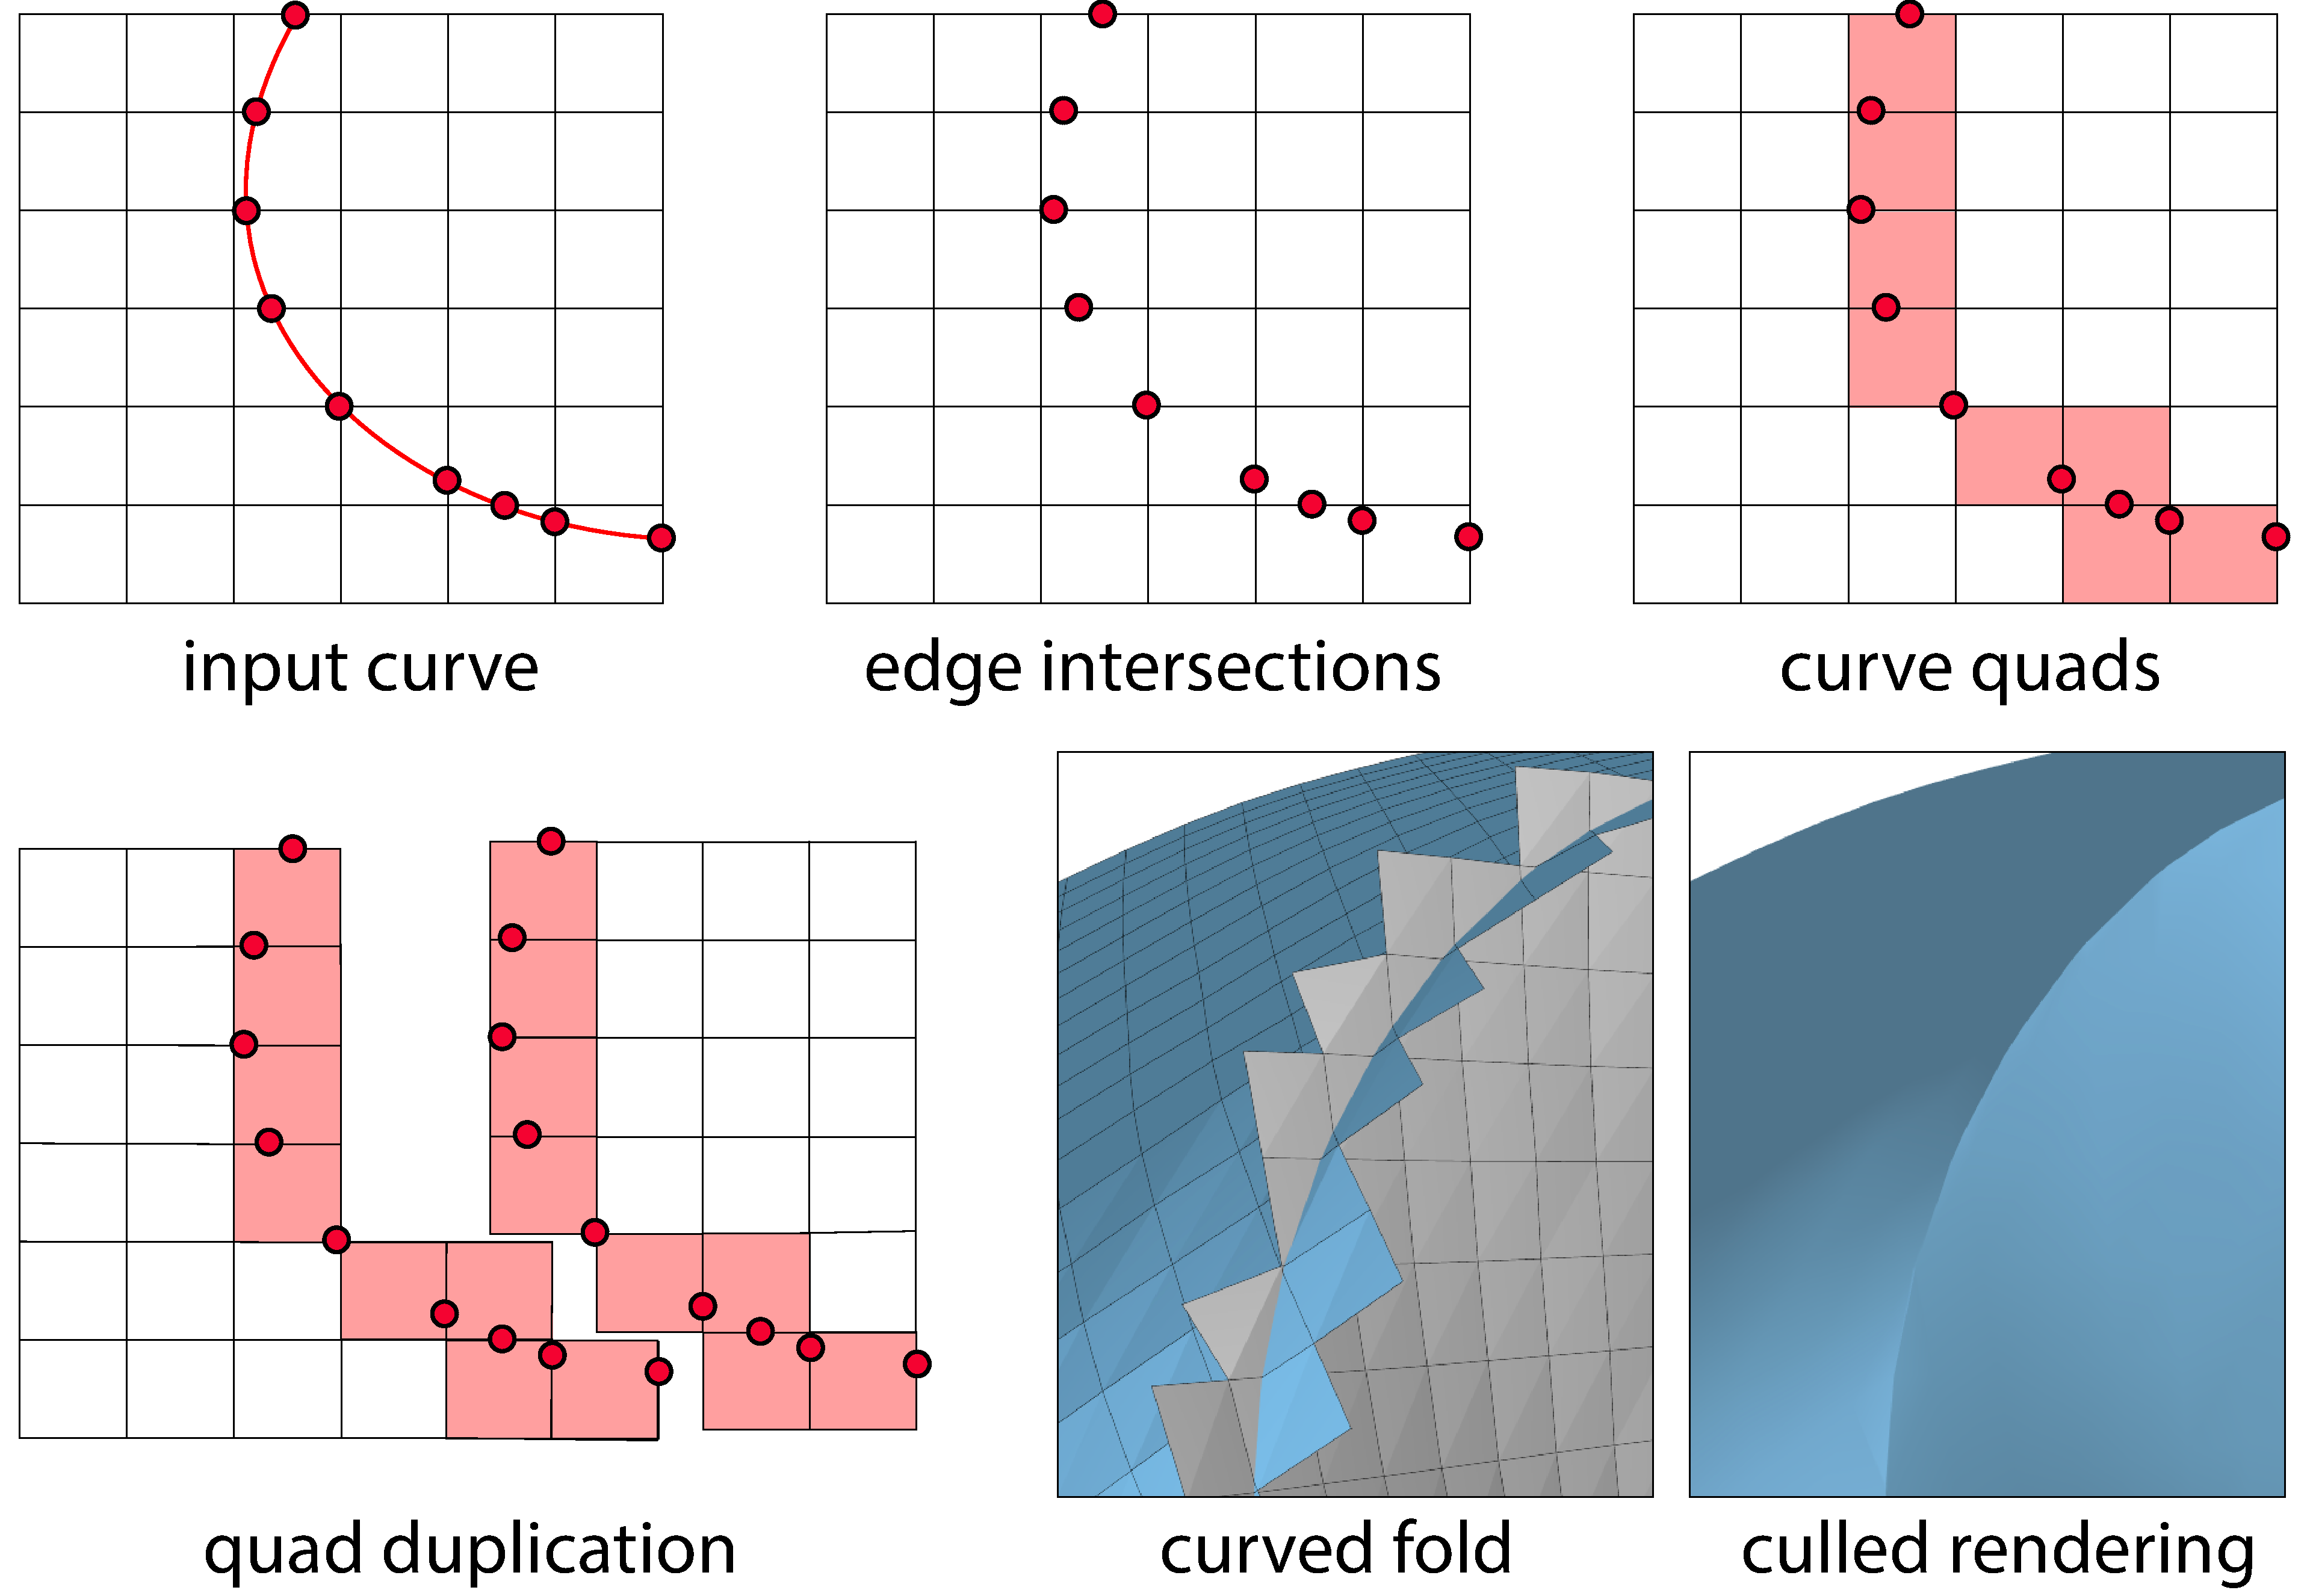
\includegraphics[width=0.8\linewidth]{figures/curve_on_dog}
	\caption{Picture taken from \cite{rabi2018shape}.}
	\label{fig:curve_on_dog}
\end{figure}

\subsection{Desiderata}
Our goal is to develop tools for the exploration of curved folded shapes on top of piecewise DOGs by means of deformations. Our choices are guided by the following ground rules for deforming DOGs:
\begin{enumerate}
  \item Perform homotopy based optimization \label{homotopy_opt}
  \item Minimally constrain DOGs \label{minimal_const}
%  \item Use accurate functionals \label{accurate_func}
%  \item Use simple functionals
\end{enumerate}
\textbf{Homotopy based optimization} is motivated both theoretically and empirically; Modeling DOGs requires solving highly constrained and non linear optimization problems, yet the theory of DOGs guarantees the existence of nearby solutions if one starts at a feasible point. In fact, generally the shape space of DOGs is a smooth manifold \cite{rabi2018shape}. This observation is worthwhile in practice; DOGs exploration was demonstrated to perform well using smooth flow, or homotopy based optimization methods both for handle based editing tasks as well for more complicated deformations such as curve-constraining flows \cite{rabi2018shape}. \\
\textbf{Minimally constrain DOGs.} As DOGs are already heavily constrained, one needs to carefully choose which quantities to constrain by hard constraints, and which ones should be optimized using soft constraints. This is essential to avoid locking, or ill-posed problems in case the constraint gradients are linearly independent \cite{rabi2018shape}. In particular, the rigidity analysis in \cite{rabi18} demonstrates that one cannot fix all edge length exactly, or likewise demand a DOG to also be a Chebyshev net. We note however that this can be done approximately and to a low tolerance as a DOG is a chebyshev at the smooth limit and at the smooth limit there is a rich set of exact isometries. The folding constraints at \secref{sec:folding} where chosen such that they could be satisfied \textit{exactly}, and so that in practice they vanish once the surface is sufficiently folded, just like a piecewise smooth curved folded surface. \\
%\textbf{Accurate functionals.} We look for constraints and objectives that are accurate and as often in the case with DOG objectives, converge under sampling of a smooth orthogonal geodesic net \cite{rabi18,rabi2018shape}. \\
%\textbf{Simple functionals.} We strongly prefer sparser objectives with a lower degree as possible. To that end, we leverage the regularity of the DOG meshing and theory on smooth orthogonal geodesic nets in our derivations. \\
\section{Fundamental tools for folding} \label{sec:folding}
In this section, we explore the different ways one can fold a given crease pattern, and derive objectives to control them.


\subsection{Curved folding from the view of the crease} \label{sec:curved_folding_from_a_curve}
Let $\Gamma(t)$ be a curve on a smooth developable surface $S$,  let $\gamma(t)$ be its flattened curve, $k(t)$ its curvature, and $k_g(t)$ its geodesic curvature such that $k_g(t) = k(t) \cos(\alpha(t))$ for some $\alpha \neq 0$. This implies that at each point along $\Gamma(t)$, the tangent planes of $S$ make an angle of $\alpha$ with the osculating planes of $\Gamma(t)$. One can switch this point of view: start with a flat curve $\gamma(t)$, isometrically embed the curve in $\mathbb{R}^3$ and construct a developable surface by reconstructing the planes at each point. As long as the crease is curved, i.e. has some normal curvature such that $k(t) > k_g(t)$ and $\alpha(t) \neq 0$ then there are 2 distinct planes containing $\Gamma'(t)$ and forming an angle of $\alpha(t)$ with the curve's osculating plane. Therefore, one can locally construct two different smooth developable surfaces passing through $\Gamma(t)$ with $\gamma(t)$ as its flattening. Alternatively, one can construct a folded surface by a consistent smooth choice of a different tangent plane for each "side" of the curve (see Fig. \ref{fig:curved_fold_through_curve}) \cite{more_on_paper}. The tangent planes from both sides are reflections of one another through the osculating plane of the curve \cite{curved_folding_kilian}.

\begin{figure} [h]
	\centering
	\includegraphics[width=0.7\linewidth]{figures/curved_fold_through_curve.pdf}
	\caption{(TODO BETTER FIG) Left: A flattened curve in 2D. Right: A small neighbourhood around an embedding of the curve in $\mathbb{R}^3$, its osculating plane and two options to extend a the curve to developable surface by constructing the 2 planes containing the curve's tangent and making an angle of $\alpha(t)$  with the osculating plane. Choosing 2 different tangents along each 'side' of the curve creates discontinuities along the curve and a curved folded surface.}
	\label{fig:curved_fold_through_curve}
\end{figure}

%Two intersecting developable surfaces can be flattened along their intersection if the intersected curve have the same geodesic curvature on both surfaces. 
\subsection{The smooth and combinatorial parameters of a single crease}
A single straight crease is rather boring, mathematically speaking. Straight lines can only be folded as in classical origami, i.e. by keeping them straight \cite{demaine_lens}. Hence the folding process of a single fold can be described by a single real number, representing the fold dihedral angle. As detailed in section \secref{sec:curved_folding_from_a_curve}, there are far more degrees of freedom for folding a curved crease; Up to rigid motion, this folding could be described by two smooth \textit{functions}: the curves' curvature $k(t) \geq k_g(t)$ and its torsion $\tau(t)$. Unlike the case of classical origami, the folding angle of a curved crease can vary along the curve. The folded shape is locally not determined only by these two smooth functions as there is an additional \textit{combinatorial} degree of freedom: the choice of a surface at each side (see \figref{fig:curved_fold_through_curve}). There are four options, two of which creates creates discontinuity along the crease. We call one folded configuration a mountain fold and the other a valley fold. %We follow \cite{demaine_lens} to distinguish between the two type of folded configurations by calling one choice a \textit{Mountain} fold and the other a \textit{Valley} fold. %We note that by \cite{demaine_lens}, a fold always consistently stays mountain/valley throughout the entire creased curve. Assuming a given normal orientation, a fold is said to be a mountain fold if the normal of the surface TODO:ADD EXPLANATION. 


%The curvature and torsion also dictates the ruling patterns of the developable surfaces, generally changing while folding and bending the surface. Deforming a curved crease locally determines the shape of both surfaces around it, and the exact regions of surfaces influenced by that fold depend on the ruling patterns themselves. As mentioned, the rulings patterns themselves can change which can smoothly change during the deformation itself. 

%(there's the cone singularity case where a curved fold is more local (as focused on the cone point) but I think this requires the curve to be C^1.. should mention it?

\subsection{The combinatorial parameters of multiple creases}
Curved folding is well understood locally, around a small part of a single curve, as the tangent planes along the curves are reflections of one another through the folded curve osculating plane. Understanding crease patterns globally still remains a challenge. In essence, deforming one patch propagates a global deformation of the patch on the other side of the crease, a process that depends on the ruling patterns. The ruling patterns are formed as the intersections of the tangent planes, and as mentioned the ruling patterns can smoothly change during the deformation itself. When there are multiple creases this process further propagate and dictates the shape of other patches (see \figref{fig:multiple_crease_pattern}). The process becomes more complicated when some creases intersect due to compatibility constraints (see \figref{fig:multiple_crease_pattern}, right figure). Generally speaking, choosing the first mountain/valley assignment of one fold dictates the mountain/valley assignments of the other folds as the location of another creased is fixed (TODO: see if I can cite demaine-tachi or if that is still unpublished). The combinatorial degrees of freedom that then remain are to determine which folds are active, i.e. folded (TODO: see figurebias-stuff).

% Can change the sentence above to not talk about mountain or valley yet, if needed.
% The pictures which will show are then discrete, though the smooth picture is the same. Maybe put the discrete picture in the setup as well.
% A fold is active if nearby tangents are reflections of one another, and is not active if they are the same as there is no discontinuity. (have a figure that is discrete, but explain it is also the same drawing for the smooth case).
% Write down the formula. Write down a flow. State it is inequality hence folding should be done at time = 0 when it is flat, but nevertheless a binary decision. We characterize it by the sign. 
% One can then view a folding-bending process as a smooth flow, i.e. a smooth deformation on a piecewise C^2 developable surface. The choice to make each fold active is only done during time t = 0, whereas otherwise discontinuties arise, and locally remains a curved fold as the equality.
% Problem in using it for a DOG is that we cannot hope to get it exactly. Then present binary representation. Say how it's really good (also goes to zero very fast).
% The binary characterization in the smooth case, motivate more degrees of freedom, and add the algorithm. Then add control for dihedral angles and mountain valley fold.

\begin{figure} [h]
	\centering
	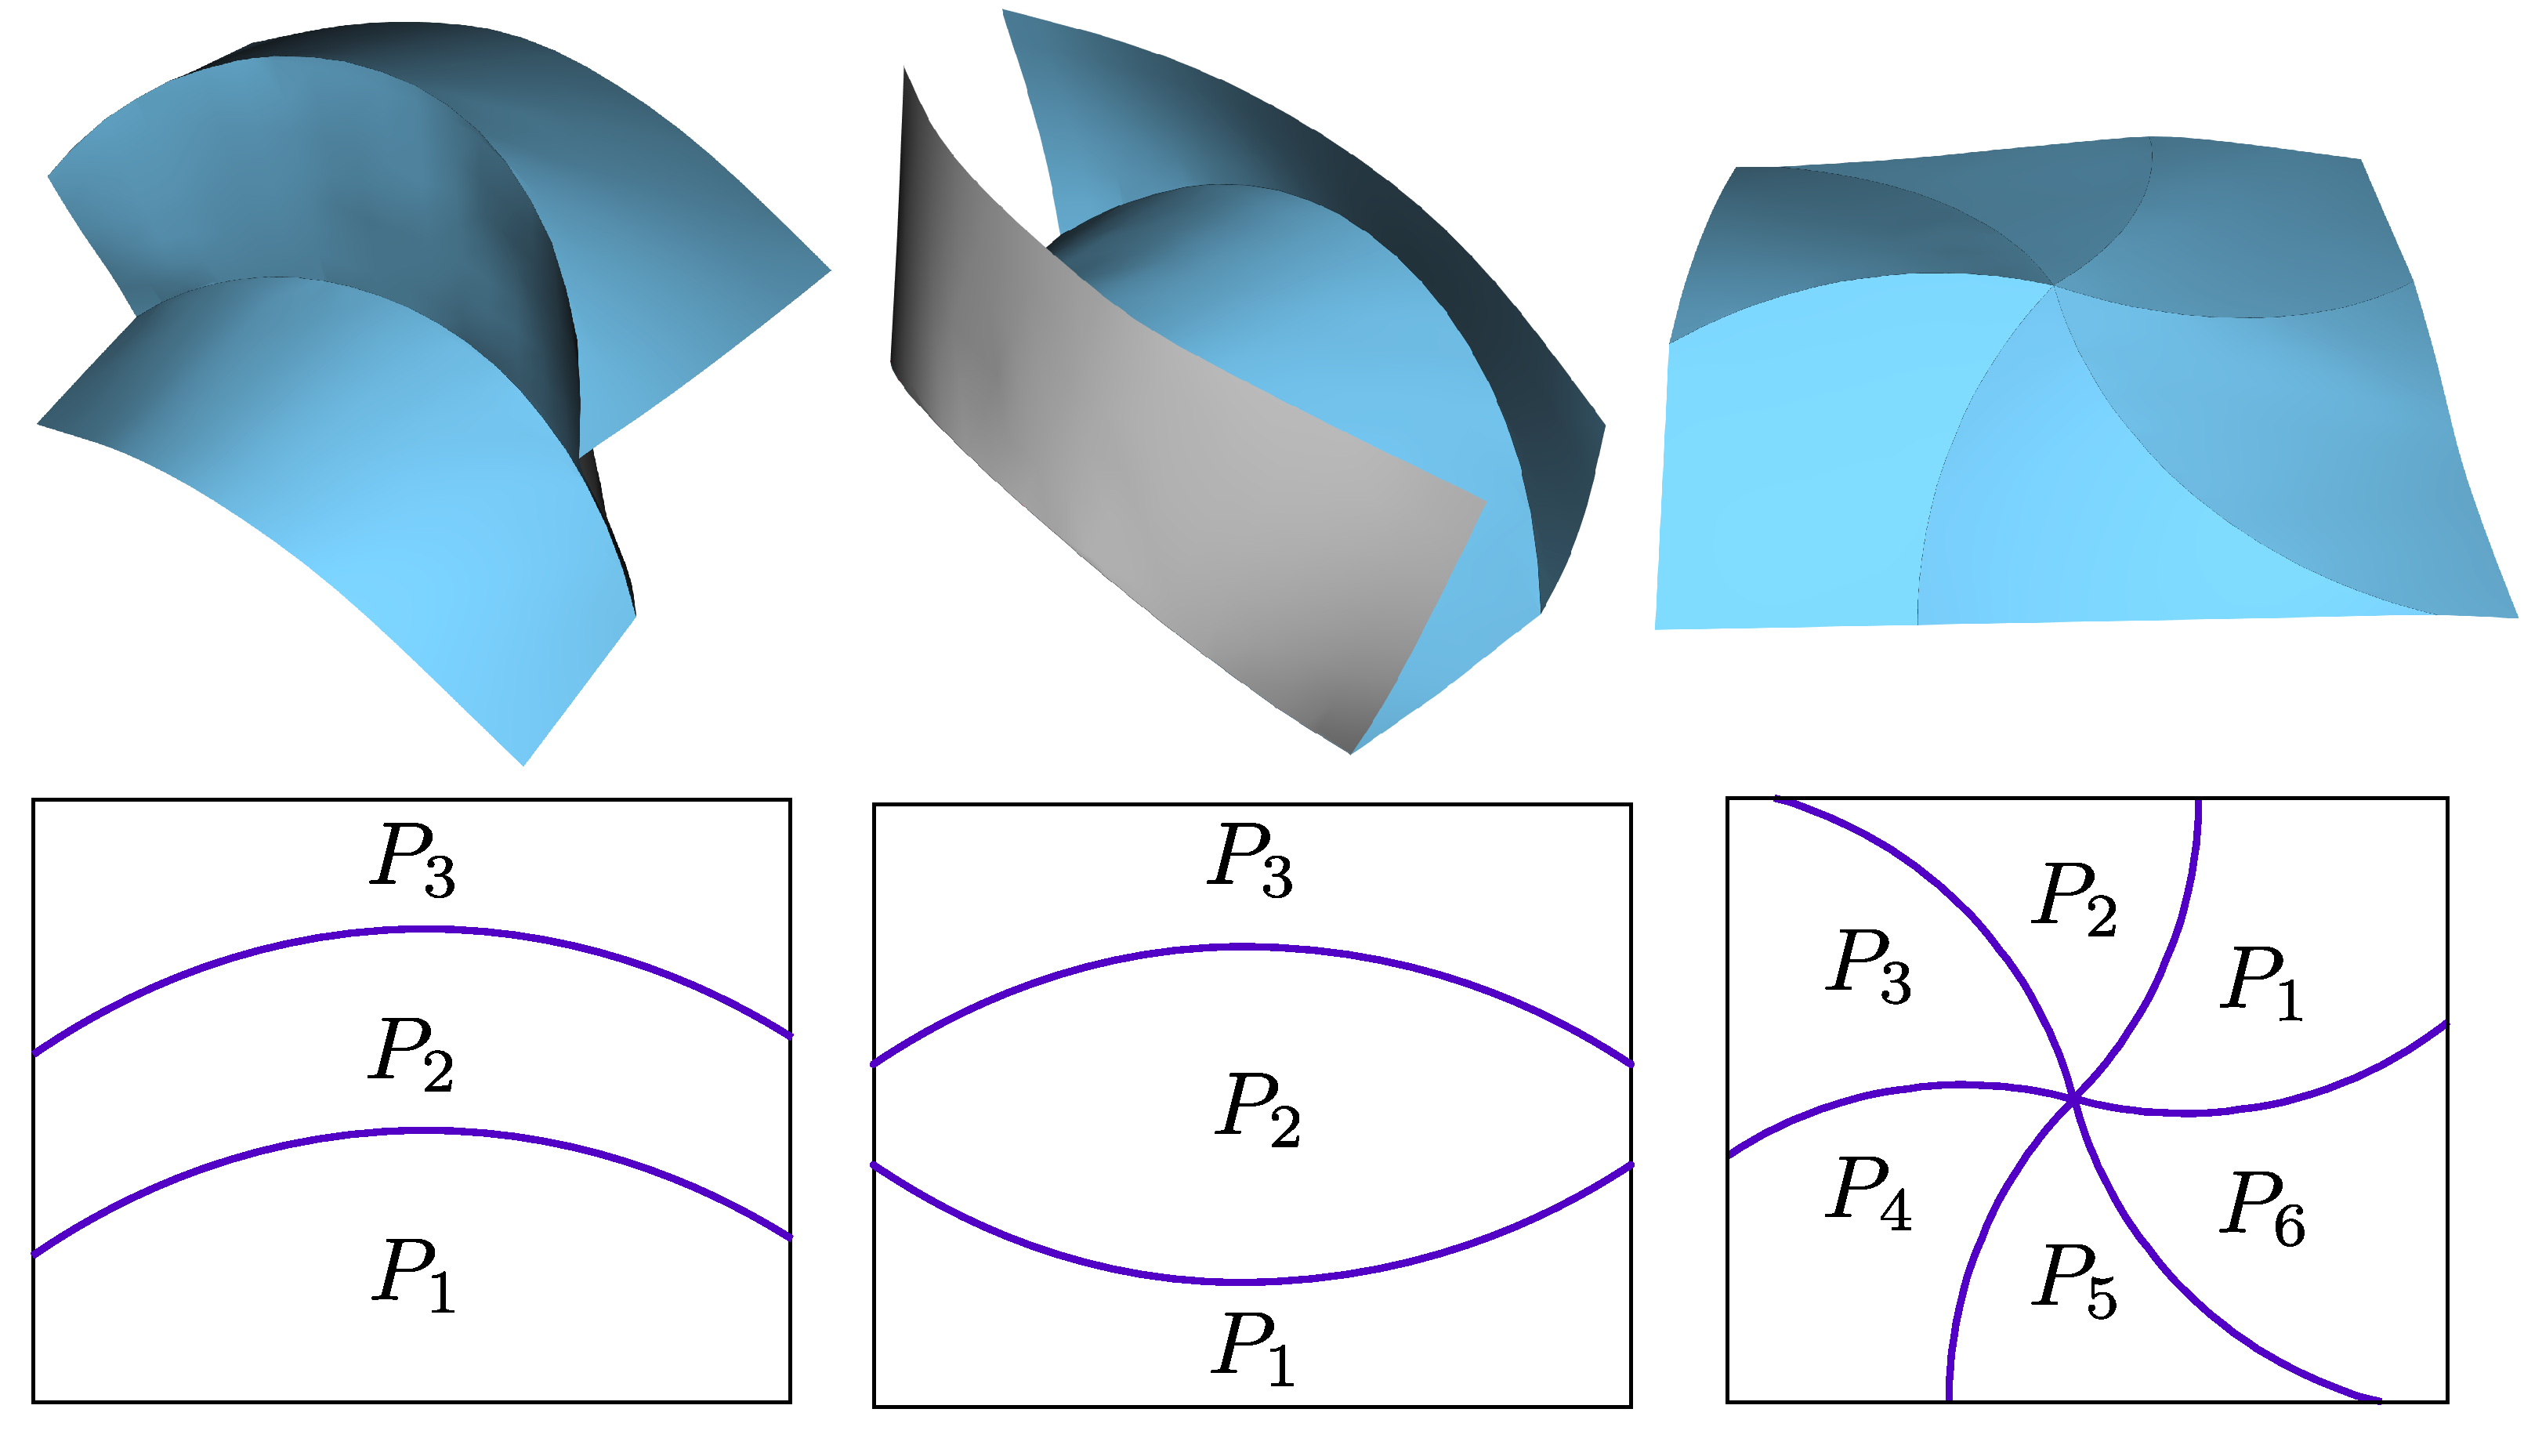
\includegraphics[width=0.7\linewidth]{figures/multiple_crease_patterns}
	\caption{Curved and straight crease patterns, decomposing a pattern into multiple components and intersecting at vertices.}
	\label{fig:multiple_crease_pattern}
\end{figure}

% !TEX root =  CurvedFoldedDogs.tex

\section{Optimization} \label{sec:implementation}
We employ \theoremref{Thm:supporting_plane} and its discretization in \equref{eq:folding_const} in a simple algorithm to enforce folding along crease curves while deforming piecewise DOGs. The algorithm aims to minimize an objective function while keeping the DOG constraints and ensuring the formation of folds along all crease curves.

\subsection{Problem setup}
We model our curved folded surfaces as a quad mesh, with a separate connected component for each patch. We denote the set of $n$ mesh vertices in $\R^3$ by $V$, the vertex positions (variables) by $\x \in \R^{3n}$, and the quad mesh faces by $F$. Each connected component is a DOG, i.e., it has the connectivity of a subset of $\Z^2$ and satisfies the DOG angle constraints \cite{rabi18}, which we denote as $\phi_{d_i}(\x) = 0, 1 \leq i \leq n$.

We are interested in deformations that fold the surface along all crease curves in a given crease pattern using \theoremref{Thm:supporting_plane} and enforcing \equref{eq:folding_const}. We enforce these constraints on all crease points, which are points on crease curves that are not crease vertices, with the exception of crease points that have the following degeneracies on the flattened mesh (see \figref{fig:fold_const_degeneracies}):
\begin{enumerate}
	\item degenerate osculating plane: crease points with a curvature smaller than a threshold $\kappa_\eps$; \label{item:deg_osc}
	\item degenerate edge: crease points on an edge, splitting it into two parts where one is shorter than $\eps_{r}$\% of the other; \label{item:deg_edge}
	\item degenerate angle with the intersecting DOG tangent: crease points where the tangent directions $t_1,t_2$ form an angle with one of the edges $e_f,e_b$ that is smaller than $\eps_\alpha$. \label{item:deg_tan_angle}
\end{enumerate}
We use the constants $\kappa_\epsilon=\text{1e-5}, \eps_r=5\%, \eps_\alpha=3^{\circ}$.

\begin{figure} [h]
	\centering
	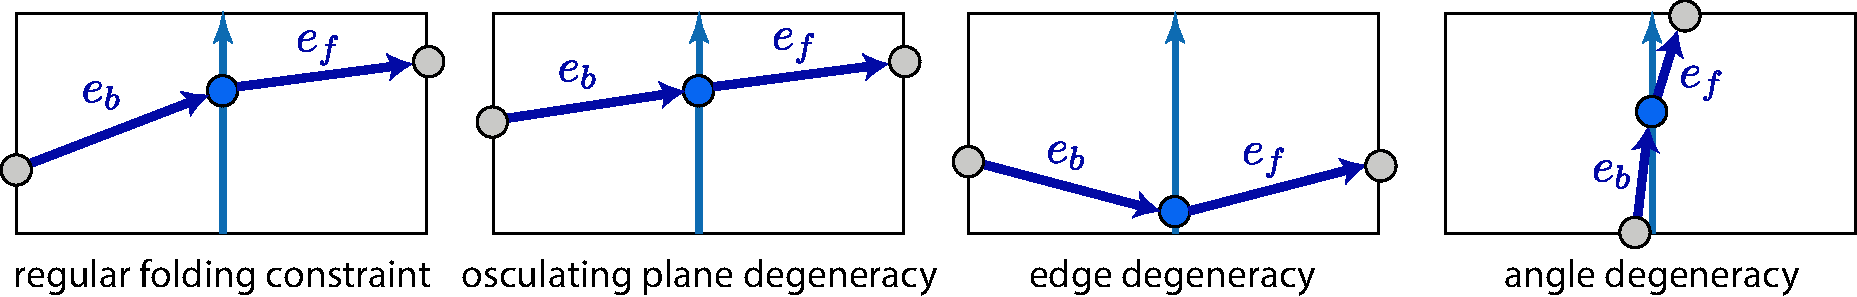
\includegraphics[width=\linewidth]{figures/fold_const_degeneracies}
	\caption{A folding edge constraint defined on a blue crease point splitting the blue edge and degenerate cases where we do not enforce the constraint. From left to right: A regular folding edge constraint, instabilities in the osculating plane's normal as $\frac{e_b \times e_f}{\|e_b \times e_f\|}$ caused by $e_b,e_f$ being almost collinear, degenerate edges as one part of the edge split by the blue crease point is comparably very short, and lastly a very small angle between $e_b$ and the DOG edge crossing the blue point. An angle degeneracy often occurs before or after an edge degeneracy.}
	\label{fig:fold_const_degeneracies}
\end{figure}

The problems we solve in this paper can be written in the form:
\begin{equation} \label{eq:const_opt}
\begin{aligned}
& \argmin_x f(x) \\
& \textrm{subject to} \\
& \phi_{d_i}(\x) = 0, \ \  i = 1, \ldots, n, \\
& \phi_{f_j}(\x) = 0, \ \  j = 1, \ldots, k, \\ 
\end{aligned}
\end{equation}
where $f$ is an objective function composed of a weighted sum of a bending objective, isometry objective, positional constraints and other terms as specified in \secref{sec:dog_obj}. \OSH{who are $\phi_{f_j}(\x)$, spell out please.}

\subsection{Folding constraints}
Motivated by the fact that in the smooth case, one cannot move from a folded to a non-folded configuration around a non-planar point, we strive to always satisfy $\phi_{f_j}(x) = 0$ exactly. The common starting point of a flat surface is an interesting case, as it is a bifurcation point between surfaces satisfying \theoremref{Thm:supporting_plane} and those that do not, which also holds for the discretization \equref{eq:folding_const_normalized}. To that end, we solve our problem with an iterative sequential quadratic programming (SQP) solver with a line search, complemented with two simple strategies to handle the folding constraints $\phi_{f_i}(\x)$:
\begin{enumerate}
	\item a penalty term \cite{nocedal} punishing  deviation from the constraints; \label{opt:penalty}
	\item a line search method that backtracks if the resulting mesh does not exactly satisfy $\phi_{d_i}(\x) = 0, i = 1,...,n$.
\end{enumerate}
Since the functions $\text{sgn}(x),H(x)$ involved in the constraints $\phi_{d_i}(\x)$ are not $C^1$, we replace them by the approximations:
%
\begin{align} 
\begin{split}\label{eq:const_inner}
&\text{sgn}(x) \approx \tanh(hx) \\
&H(x) \approx  \left\{\begin{array}{@{}l@{\thinspace}l}
0  &: \text{if } x \leq 0, \\
\frac{x^2}{x^2+\delta} &: \text{if } x = 0, \delta > 0 \\
\end{array}\right.
\end{split}
\end{align}
using the fixed parameters $h=1000,\delta = \text{1e-5}$. Our approximation for $H(x)$ is taken from \cite{l0_approximation,autocuts}.  The use in a homotopy based optimization necessitates an approximation for $H(x)$ that vanishes on a flat mesh, and therefore we do not use the common approximation for the Heaviside function $H(x) \approx \hat{H}(x) =  \frac{1+\tanh(hx)}{2}$ because $\hat H(0) = \frac{1}{2}$.

We refer to the approximated constraints as $\phi^*_i(\x)$ and replace the optimization problem \eqref{eq:const_opt} with the following problem:
\begin{equation} \label{eq:const_opt_penalty}
\begin{aligned}
& \argmin_x f(x) + \omega \sum \|\phi^*_{f_j}(\x)\|_2^2 \\
& \textrm{subject to} \\
& \phi_{d_i}(\x) = 0, \ \  i = 1, \ldots, n. \\ 
\end{aligned}
\end{equation}
Here, $\omega > 0$ is a metaparameter initialized as $\omega_0 = 1$ and which doubles its value if the line search cannot find a point that both decreases a given merit function while satisfying the supporting plane conditions exactly. In practice, the penalty term only affects points that are very close to being planar, while approaching zero very quickly around already folded points.

\subsection{Equality constrainted SQP}
For ease of notation, we use the following notation to refer to the objective of \eqref{eq:const_opt_penalty}:
\begin{equation}
f_\omega(\x) = f(x) + \omega \sum \|\phi^*_{f_i}(\x)\|_2^2
\end{equation}
We minimize \eqref{eq:const_opt_penalty} using an iterative Sequential Quadratic Programming (SQP) solver with a linesearch \cite{nocedal}. Given a set of variables at a given iteration $x^k$ and current values of lagrange multipliers $\lambda^k$, a linesearch equality constrained SQP algorithm iteratively find the next direction for a linesearch of \eqref{eq:const_opt_penalty} by which it sets the next variables $x^{k+1}$ by solving a KKT system of the form:

\begin{equation} \label{eq:KKT_eps}
\begin{gathered}
{K} \begin{pmatrix} d^{k+1} \\ \lambda^{k+1} \end{pmatrix}=\mathbf{b} \\
{K}=\begin{pmatrix}
{\Delta^2_{xx}\mathcal{L}(x^k,\lambda^k)} & {J^\tr}(\x^k)\\
{J(\x^k)} &  0 \\
\end{pmatrix}, \ \ 
\mathbf{b}=\begin{pmatrix}
{\nabla f_\omega(x^k)} \\ 
-\phi_{d_i}(x^k)\\
\end{pmatrix}.
\end{gathered}
\end{equation}

Where $J(\x)$ is the Jacobian of the equality constraints in \eqref{eq:const_opt_penalty}, $\Delta^2_{xx}\mathcal{L}(x,\lambda) = H_{f_\omega}(x)+\sum\lambda_i^{k} \nabla \phi_{d_i}(x)$ is the Lagrangian of the problem and $H_{f_\omega}(\x)$ is the Hessian of $f_\alpha(\x)$.

Following \cite{rabi2018shape}, we use a minimally modified Jacobian $J^*(x)$ to deal with singularities in DOGs. We also replaced the Hessian of the objective $H_{f_\alpha}(\x)$ by a convex approximation which we denote by $H^*_{f_\omega}(\x)$, as detailed in \ref{sec:dog_obj}, and thus replace the system \eqref{eq:KKT_eps} by:

\begin{equation} \label{eq:KKT_us}
\begin{gathered}
{K} \begin{pmatrix} d^{k+1} \\ \lambda^{k+1} \end{pmatrix}=\mathbf{b} \\
{K}=\begin{pmatrix}
{ H^*_{f_\omega}(\x^k)+\sum\lambda_i^{k} \nabla \phi_{d_i}(\x^k)} & {J^{*^\tr}(\x^k)}\\
{J^*(\x^k)} &  0 \\
\end{pmatrix}, \ \ 
\mathbf{b}=\begin{pmatrix}
{\nabla f_\omega(x^k)} \\ 
-\phi_{d_i}(x^k)\\
\end{pmatrix}.
\end{gathered}
\end{equation}

We note that at \cite{rabi2018shape} the authors discretized Laplacian metric flows by solving a similar system with a Laplacian instead of the objectives' Lagrangian, however we found that replacing the Laplacian by the Lagrangian followed by convexifying the Hessian performs significantly better, especially on larger models. As common in SQP algorithms, our linesearch used a merit function defined as a combination of the objective and the constraints, thus the linesearch chooses step sizes that both reduce the objective and keep the constraints numerically feasible. This removed the need of the slower LBFGS constraints projection used by \cite{rabi18,rabi2018shape}. We used the L2 merit function \cite{nocedal}:
\begin{equation}
\psi(\x;\mu) = f_\alpha(\x)+\mu\sum\|\phi_{d_i}(x)\|_2
\end{equation}
where we update the parameter $\mu^k$ at each iteration using the absolute values of the Lagrange multipliers \cite{nocedal}:
\begin{equation}
\max(c_\mu \max(\{\abs{\lambda_i^k}\}), \mu_0)	
\end{equation}
with $c_\mu = 1.1$ and $\mu_0 = 0.05$.

\subsection{Objectives and constraints} \label{sec:dog_obj}
Our object $f$ is composed of a weighted sum of various functions measuring bending, stretch, positional constraints and dihedral angles.
We use an integrated sqaured mean curvature bending objective taken from \cite{rabi2018shape}, but exploit the fact that it is quadratic and convex under isometric deformations (\cite{quadratic_bending}):
\begin{equation}
f_\text{H}(\x) = 0.5\x^t(L^tM^{-1}L)\x
\end{equation}
Where $L$ is the DOG Laplacian and $M$ is a diagonal mass matrix defined by the DOG vertex area \cite{rabi2018shape}. \\
Let $c^i$ be a crease point, $t_1^i$ and $t_2^i$ the grid tangents as in \figref{fig:fold_angle_and_tangent_angles}, and let $\theta^i$ be a desired dihedral angle along the fold at $c^i$. Let $t^i$ be the tangent of the curve of the flat mesh at the crease point $c_i$ where we discretize $t^i$ as the tangent of the unique circle passing through $c_i$ and its neighbours on the crease. Let $cos(\alpha^i) = \langle t^i,t_1^i \rangle = \langle t^i,t_2^i \rangle$ on the initial flat mesh. We employ \lemmaref{lem:tangents_dihedral} to constrain the fold dihedral angle at $c(i)$ using a soft penalty:
\begin{equation}
\phi_{\text{d}_{c^i}}(\x) = \langle t_1^i, t_2^i \rangle - cos(\alpha)^2 - sin^2(\alpha^i) cos(\theta^i)
\end{equation}
And note that under isometry deformations $t_1,t_2$ are linear in the vertices locations, $\alpha$ is fixed, and the constraint is quadratic. Throughout the optimization we enforce a given dihedral angle constraint in an homotopy fashion by linearly interpolating the constrained angle from zero to the user requested value. \\
Let $e$ be an edge on the mesh, $l_e$ its length and $l_e^0$ the length in a reference mesh. We define the following quadratic isometry constraints:
\begin{equation}
\phi_\text{iso}(\x)_e = l_e^2 - {l_e^0}^2
\end{equation}
The patches themselves also need to align along the creases as detailed at \ref{sec:model}, which can be enforced by linear constraints as done in \cite{rabi2018shape} which we denote by $\phi_\text{a}(\x)$. We enforce the dihedral, positional, isometry and patches alignment constraints as positional constraints in a soft manner by using a penalty on their squared deviation, denoted accordingly by $f_\text{d}(\x)$,$f_\text{pos}(\x)$,$f_\text{iso}(\x)$,$f_\text{a}(\x)$. We use the constraints Gauss-Newton's Hessian as a convex approximation for the Hessian of these constraints as well as the hessian of the folding constraints  $\sum \|\phi^*_{f_i}(\x)\|_2^2$. Isometry is enforced as a soft constraint $f_\text{iso}(\x)$, as advised by the degrees of freedom analysis in \cite{rabi18,rabi2018shape}, but we emphasis that all of our results have an averaged relative edge stretch that is less than $0.003$, and a maximum stretch below $4$. As opposed to \cite{rabi2018shape} we also encode  $\phi_\text{a}(\x)$ as a soft constraint, as we have noticed a significance improvement in the quality and smoothness of complicated crease patterns when these are enforced as a soft penalty with a large weight \MiR{ok to say?, this is mostly important in the curved constrained case for interactivity, as if we run the interpolation much slower then we can still use hard constraints},  with an average deviation of $0.0002$ and a maximum of $0.0035$. We note that the constrained shape space analysis in \cite{rabi2018shape} only concerns the DOG angle constraints, and complicated crease patterns rise to a large set of additional linear constraints.\\ 
The objective we optimize is then:
\begin{equation}
f(\x) = w_Hf_\text{H}+w_pf_\text{pos}+w_df_\text{d}+w_{iso}f_\text{iso}+w_af_\text{stitching}
\end{equation}
Throughout the paper, unless stated otherwise, we use $w_H = 1$, $w_{pos}=5$,$w_d = 100$, $w_{iso}= \frac{20000}{\|E\|}$, $w_a = 1e4$. Where $\|E\|$ is the number of edges in the mesh (i.e. for a mesh with $1000$ vertices $w_{iso}=20$). Our meshes are always scaled to have an average edge length of $1$ and therefore using a different resolution for the same geoemtry keeps our bending objective the same, however scales the isometric objective by the number of edges.
\section{Results} \label{sec:results}
\MiR{We use CGAL's arrangement model \cite{cgal,cgal_arr1,cgal_arr2} to compute a given planar arrangement from an input polyline, Paradiso (cite) to solve our linear systems), and libigl for other stuff. In our optimization we enforce a given dihedral angle constraint in an homotopy fashion by linearly interpolating the constrained angle from zero to $\theta^i$. Curve constrained stuff. \\}

%For rendering purposes, we keep another mesh where the extraneous parts of the duplicated faces are culled.
\subsection{Editing system}
\MiR{Important: Enforcing the folding constraint automatically choose M/V assignment (show figure). Also write it down in figures.}
\begin{figure} [h]
	\centering
	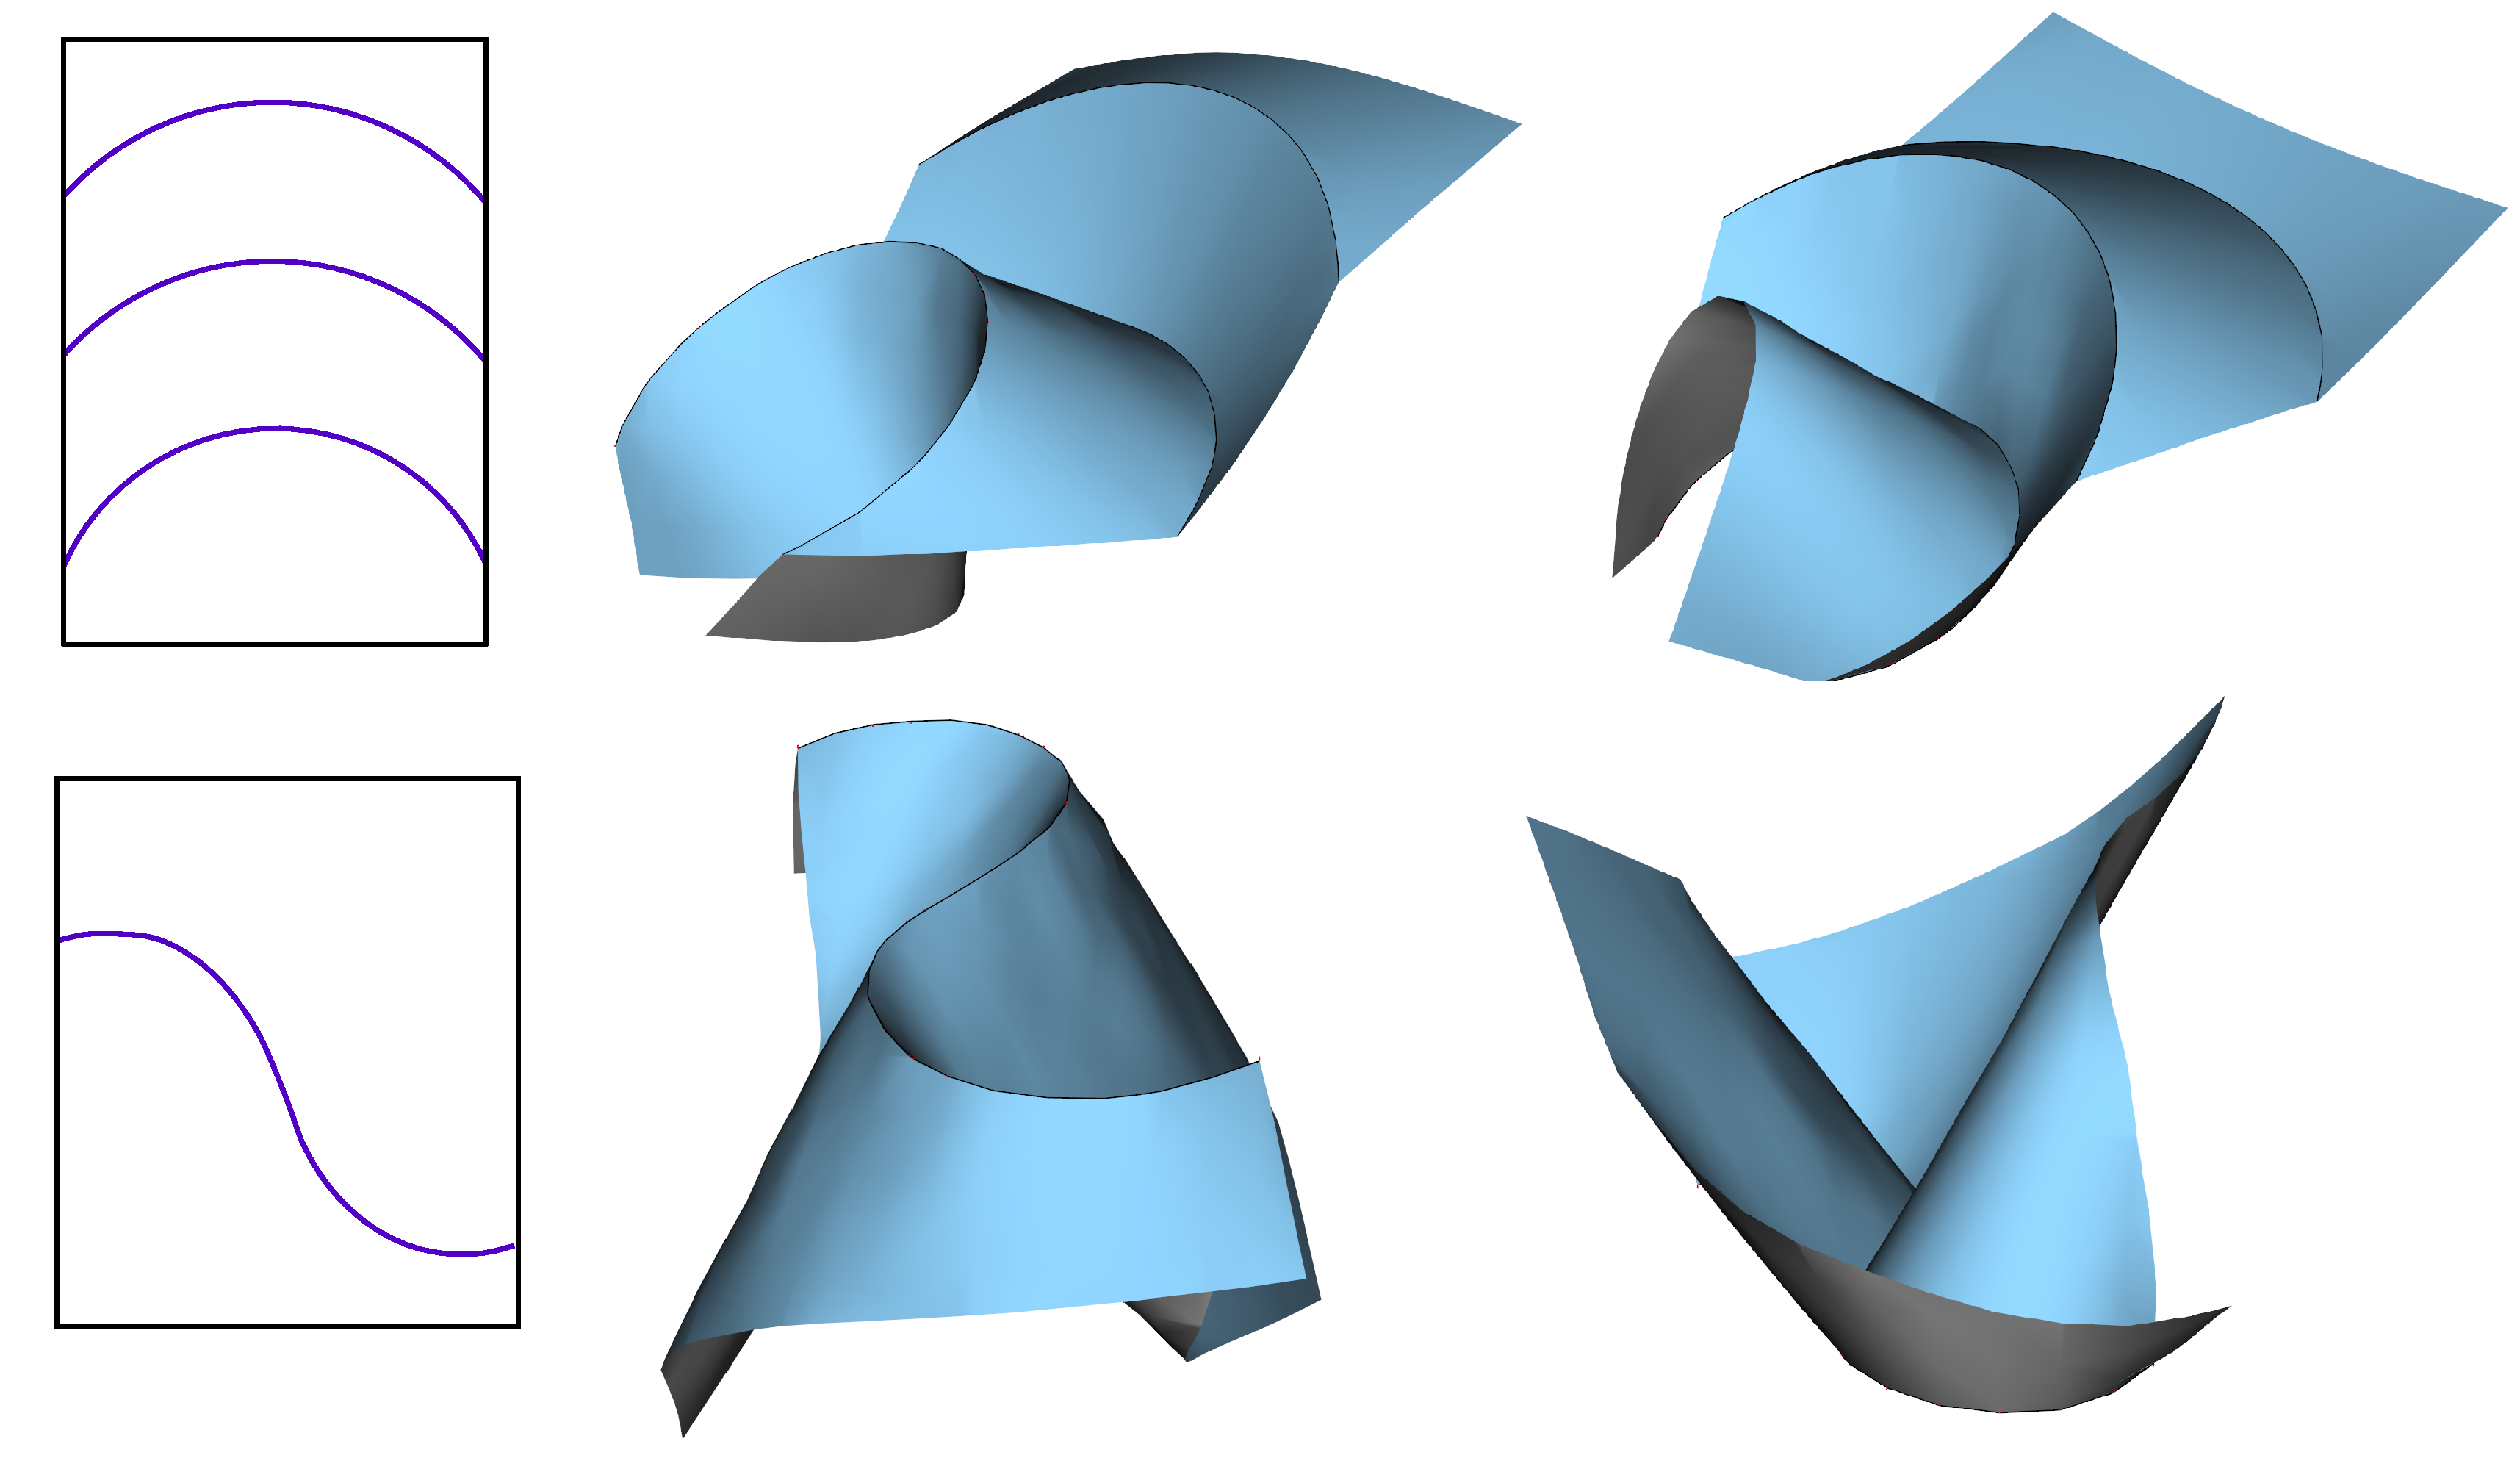
\includegraphics[width=\linewidth]{figures/MV_bias_modeling}
	\caption{\MiR{Same pattern, same curve deformation, different mountain/valley assignment by enforcing constraint \eqref{eq:mountain_valley} along the fold.}}
	\label{fig:MV_bias_modeling}
\end{figure}

\begin{figure} [h]
	\centering
	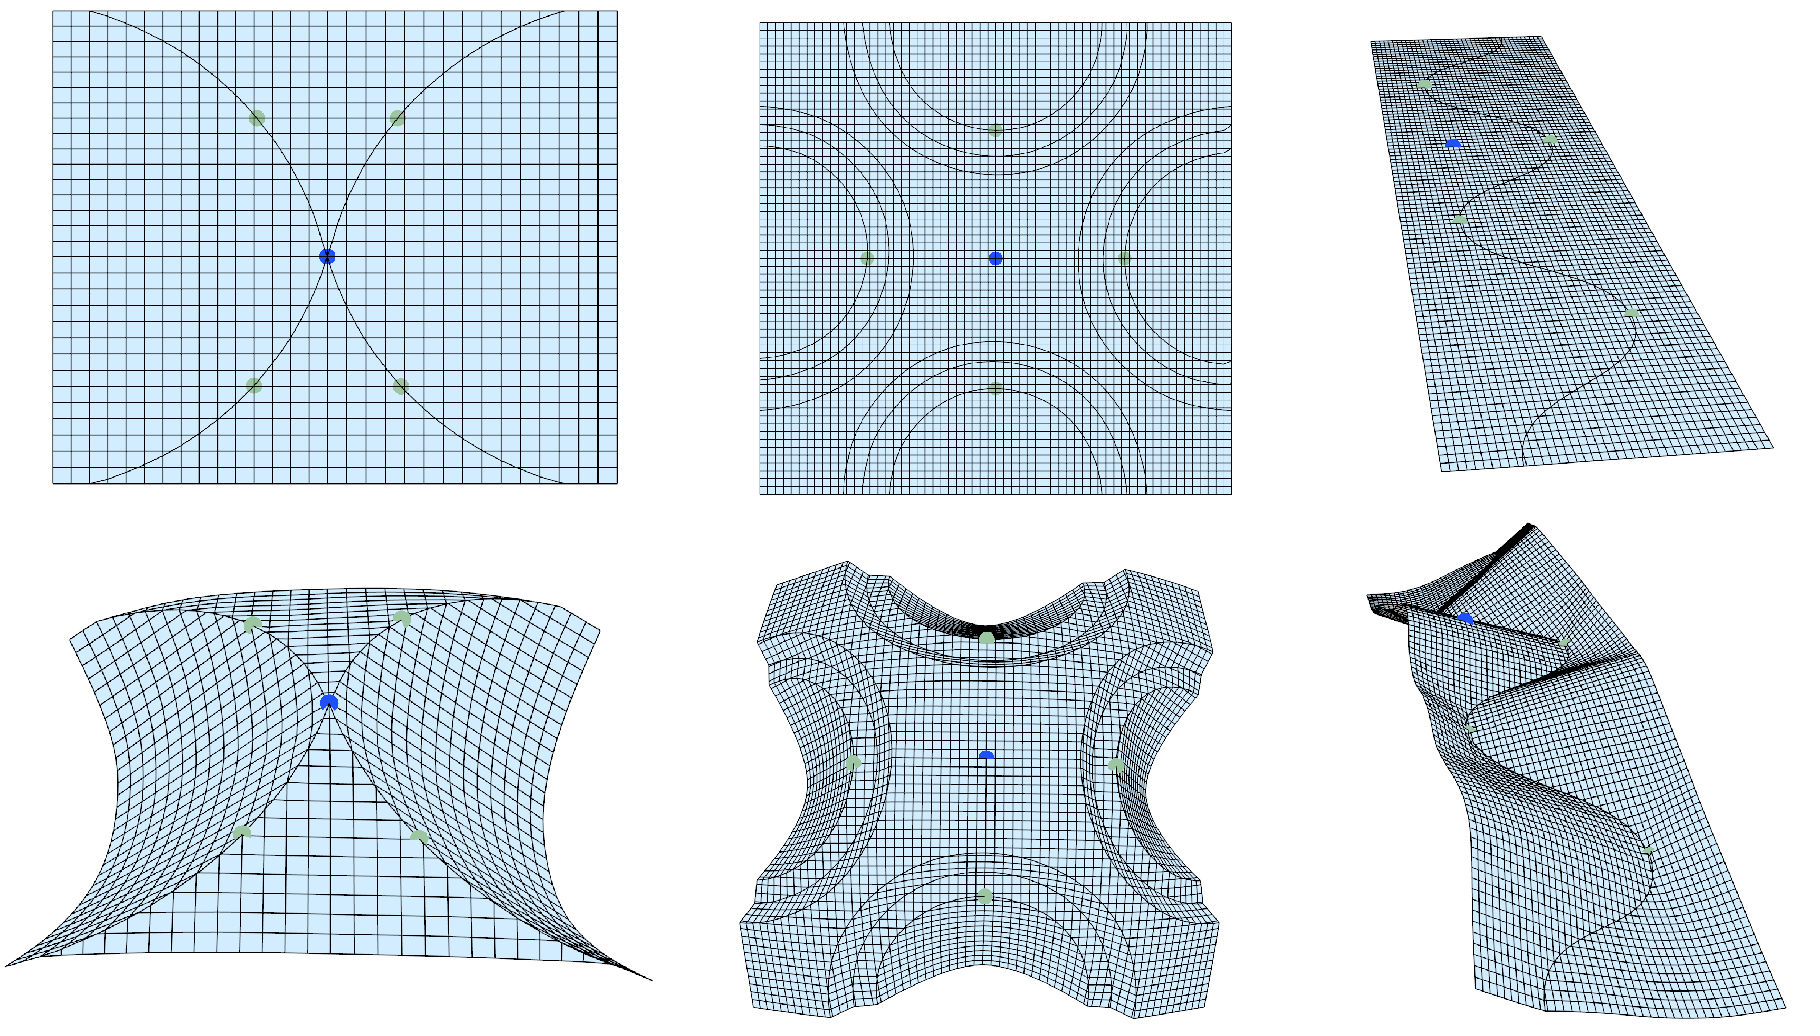
\includegraphics[width=\linewidth]{figures/dihedral_editing}
	\caption{\MiR{Dihedral angle, homotopy.}}
	\label{fig:dihedral_editing}
\end{figure}
\section{Conclusions and future work}
This paper is a first step towards unhindered freeform modeling of curved folded surfaces. Basing our models on DOGs \shortcite{rabi18} allows us to capture the full set of curved folded deformations, and our discretization in \secref{sec:folding} together with the folding algorithm in \secref{sec:implementation} allows us to steer the modeled deformations towards those that simultaneously fold and bend crease curves. Our deformation algorithm is able to model bending and folding of complicated crease patterns by merely using positional constraints, making it highly suited for exploration of new curved folded surfaces. We supply further optional objectives to constrain dihedral angles and mountain/valley assignment in \secref{sec:folding_angles_mountain_valley}, giving designers additional expressiveness. \\
Similar to other works on modeling DOGs \shortcite{rabi18,rabi2018shape}, the most obvious limitation of our algorithm is speed. Our optimization framework allows us to interactively model up to $2000$ vertices. We leave scaling of the optimization to future work, possibly by using a multigrid solver on the DOG grids. Throughout the design, we found that we lacked tools and objectives to enforce symmetry. In particular, we would like to look at folding of curved symmetric plane wallpappers and tessellations \cite{demaine_lens,mundilova2019mathematical}. Finally, we note that we model deformations of a given fixed input crease pattern. Optimizing and changing an input crease pattern, as done in origami modeling tools \cite{tachi2010freeform}, could offer new and exciting ways to discover and design curved folded surfaces. 

\begin{acks}
The authors would like to thank Oliver Glauser, Justin Solomon, Martin Kilian and Niloy Mitra for illuminating discussions, Katja Wolff and Phillip Herholtz with results and figures production. The work was supported in part by the Deutsche Forschungsgemeinschaft-Collaborative Research Center, TRR 109, ``Discretization in Geometry and Dynamics'' and a gift from Facebook, Adobe and Snap, Inc.
\end{acks}

% Bibliography
\bibliographystyle{ACM-Reference-Format}
\bibliography{CurvedFoldedDogs}

\appendix


\end{document}